\chapter{Grundlagen}
\label{cha:Grundlagen}

In diesem Kapitel werden verschiedene Konzepte der Spieltheorie Abschnitt \ref{sec:Spiele mit Gegner} und des maschinellen Lernens Abschnitt \ref{sec:Verstärkendes Lernen} genauer erklärt und veranschaulicht. Diese Konzepte sind der Grundbaustein für die spätere Anwendung der lernfähigen Verfahren. Konzepte der Spieltheorie sind z.B. Suchstrategien und deren Optimierungen. Im zweite Abschnitt "Verstärkendes Lernen" behandeln wir das Konzept eines Agenten der ohne Strategie in einer Welt ausgesetzt wird und in dieser Aktionen ausführt. Wir betrachten insbesondere das Verhalten des Agenten hinsichtlich einer Belohnung für eine durchgeführte Aktion. 

\section{Spiele mit Gegenspieler}
\label{sec:Spiele mit Gegner}
Schach, Vier Gewinnt, Dame, Tic Tac Toe und Reversi sind strategische Spiele für zwei Personen, die gegeneinander antreten, um nach den Regeln des Spiels, den Gegenspieler zu besiegen. Diese Spiele sind deterministisch weil, dass Spiel nicht vom Zufall abhängt und der gleiche Spielzug führt bei gleichem Ausgangszustand immer zum selben Zustandsübergang. Zudem sind sie überschaubar weil, zu jedem Zeitpunkt des Spiels das Spielfeld und alle Spielzüge einsehbar sind. Ein nichtdeterministisches Spiel mit Gegenspieler ist z.B. Backgammon, denn Würfelergebnisse und somit der Zufall sind Bestandteil des Spiels. Wie kann ein Programm einen Menschen in einem dieser Strategiespiele besiegen? In den nachfolgenden Unterabschnitten werden Konzepte der Spieltheorie erläutert, die versuchen diese Frage zu beantworten.

\myparagraph{Nullsummenspiele} 
Ein Nullsummenspiel ist ein Spiel bei dem der Verlust eines Spielers einen gleich hohen Gewinn für den Gegenspieler bedeutet. Gewinnt ein Spieler eine Partie eines Nullsummenspiels, dann verliert der Gegenspieler automatisch. Der gewinnende Spieler erhält einen Pluspunkt und der verlierende Spieler einen Minuspunkt. Die Summe der beiden Ergebnisse ist Null. Gewinnt beziehungsweise verliert keiner der beiden Spieler, dann erhalten beide Spieler als Spielergebnis eine Null. Die Summe der beiden Ergebnisse ist wiederum Null, so lässt sich der Name "Nullsummenspiele" herleiten. Die beiden Spiele Tic Tac Toe und Reversi sind Nullsummenspiele. 

\subsection{Minimax}
Ein Spieler wird als MAX bezeichnet und der Gegenspieler als MIN. Spieler MAX versucht einen maximalen Gewinn für sich zu erlangen und Spieler MIN versucht den erreichbaren Gewinn von MAX zu minimieren. Es wäre auch möglich anzunehmen, dass Spieler MIN einfach irgendeinen zufälligen oder dummen Spielzug auswählt und MAX einen einfachen Sieg erlangt. Diese Annahme entspricht jedoch wenig einem realen Spiel, bei dem beide Spieler versuchen das Spiel zu gewinnen.\\

In Abbildung \ref{fig:minimax_tictactoe} ist der Ablauf einer Minimax-Suche veranschaulicht. Der Minimax-Suchbaum berücksichtigt jeden Zustand indem sich die Spielwelt befinden kann. Im ersten Spielzug könnte Spieler MAX sein Kreuzspielstein in die obere linke Ecke setzen, daraus ergeben sich neue Zustandsmöglichkeiten. Spieler MIN könnte seinen Kreisspielstein ein Feld weiter rechts und in die selbe Reihe wie Spieler MAX setzen. Der Nutzen der einzelnen Züge ist zur Zeit der Ausführung noch nicht bekannt, erste wenn das Tic Tac Toe Spiel einen Endzustand erreicht, werden den Spielern ihre Spielergebnisse mitgeteilt. Der Minmax-Suchbaum ist somit rekursiv zu betrachten. Von seinen Blattknoten ausgehend entscheidet sich MIN für den geringsten Nutzwert und MAX für den höchsten. Die Entscheidungen stehen in direkter Abhängigkeit zur vorherigen Entscheidung des Gegenspielers. \\
  
\begin{figure}[!htbp]
  \centering
  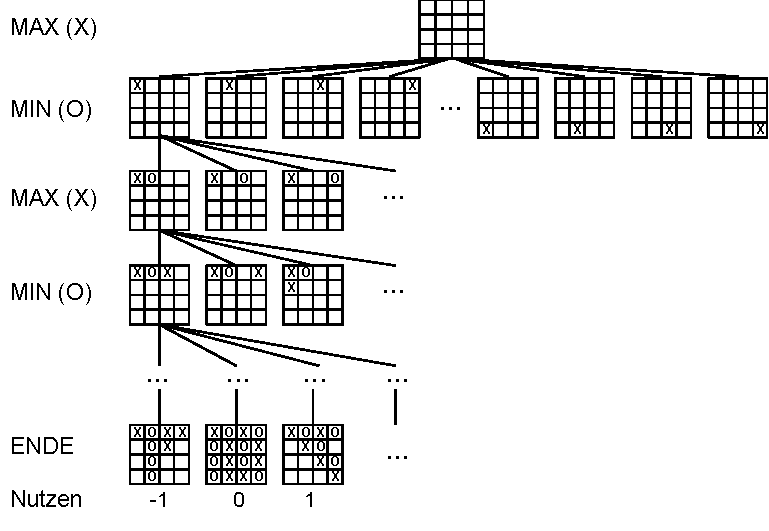
\includegraphics{inhalt/abbildungen/minimax_tictactoe.pdf}
  \caption{Ein (partieller) Suchbaum vgl. Abbildung 5.1 \cite[208]{Russell}}
  \label{fig:minimax_tictactoe}
\end{figure} 

Das größte Problem der Minimax-Suche ist die exponentielle Vergrößerung der Anzahl der Blattknoten des Suchbaums, schon bei sehr einfachen Spielen z.B. einem 3x3 Tic Tac Toe mit Neun Spielfeldern ist der Suchbaum bereits sehr groß ungefähr 362880 Blattknoten mit einem effektiven Verzweigungsfaktor von Neun der sich nach jedem Halbzug um Eins verringert. Erweitern wir die Dimension des Tic Tac Toe Spiels, so erhalten wir ein 4x4 Tic Tac Toe Spiel mit 16 Spielfeldern, einem Verzweigungsfaktor von 16 und ungefähr 20922789888000 Blattknoten. Der effektive Verzweigungsfaktor beim Schach liegt etwa bei 30 bis 35. Bei einem typischen Spiel mit 50 Zügen pro Spieler hat der Suchbaum dann mehr als $30^{100} \approx 10^{148}$ Blattknoten\cite[114]{Ertel}. Der Minimax-Algorithmus ist, auf Grund enormer Rechenzeit, in seiner Reinform praktisch nicht anwendbar, daher werden wir Erweiterungen der Minmax-Suche und andere Konzepte kennen lernen.

\subsection{Alpha-Beta-Pruning}
Eine Möglichkeit die Rechenzeit der Minimax-Suche zu verbessern ist das Kürzen oder Beschneiden des Suchbaums(eng. Pruning). Beim Alpha-Beta-Kürzen wird der Teil des Suchbaums beschnitten, der keinen Effekt auf das Ergebnis der Minimax Suche hat. Der Minimax Algorithmus wird um zwei Parameter Alpha und Beta ergänzt. Die Bewertung erfolgt an jedem Blattknoten des Suchbaums. Alpha enthält den aktuell größten Wert, für jeden Maximum Knoten, der bisher bei der Traversierung des Suchbaums gefunden wurde. In Beta wird für jeden Minimum Knoten der bisher kleinste gefundene Wert gespeichert. Ist Beta an einem Minimum Knoten kleiner oder gleich Alpha ($Beta \leq Alpha$), so kann die Suche unterhalb von diesem Minimum Knoten abgebrochen werden. Ist Alpha an einem Maximum Knoten größer oder gleich Beta ($Alpha \geq Beta$), so kann die Suche unterhalb von diesem Maximum Knoten abgebrochen werden \cite[116]{Ertel}. \\

\begin{figure}[!htbp]
  \centering
  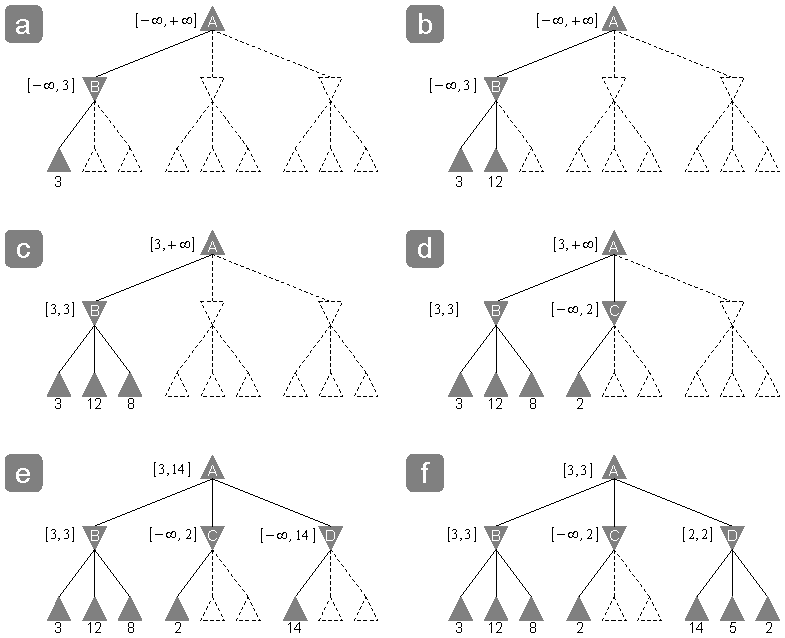
\includegraphics[scale = 0.8]{inhalt/abbildungen/alpha_beta_suchbaum.pdf}
  \caption{Ein Alpha Beta Suchbaum \cite[213]{Russell}.}
  \label{fig:minimax_tictactoe}
\end{figure} 

Verdeutlichen wir das Alpha-Beta-Pruning an Hand eines Beispiels aus dem Standardwerk der künstlichen Intelligenz von S. Russell und P. Norvig Abbildung 5.5 \cite[213]{Russell}. Ein Dreieck mit der Spitze nach oben ist ein Maximumknoten und ein Dreieck mit der Spitze nach unten ist ein Minimumknoten. Leere Dreiecke ohne einen bezeichnenden Buchstaben und gestrichelter Umrandung sind noch nicht explorierte Knoten. Durchgängige Linien verweisen auf bereits besuchte Pfade und gestrichelte Linien verweisen auf noch nicht besuchte Pfade. Die Zahlen unterhalb der Blattknoten sind die Nutzwerte die der maximierende Spieler erhält, wenn er den Pfad bis zu diesem Blattknoten durchschreitet. \\

(a) Minimum Knoten B findet einen Nutzwert 3, da dieser Wert der bisher kleinste gefundene Wert ist wird er in Beta gespeichert. \\

(b) Der Minimum Knoten B exploriert einen zweiten möglichen Nutzwert 12. Dieser Wert ist höher als der vorher gefundene und in Beta gespeicherte Wert 3, daher wird der minimierende Spieler versuchen diesen Nutzwert für den maximierenden Spieler zu vermeiden. Der neue Wert wird vom Minimum Knoten B ignoriert und Beta bleibt unverändert. \\

(c) Minimum Knoten B findet den Wert 8, dieser ist genau wie 12 größer als 3 und daher wird Spieler MIN vermeiden, dass Spieler MAX zu diesem Spielergebnis gelangt. Minimum Knoten B hat alle seine nachfolgenden Knoten exploriert. Maximum Knoten A wird vom Minimum Knoten B maximal den Nutzwert 3 erhalten, somit ergibt sich für den Maximum Knoten A, dass dieser mindestens den Nutzwert 3 erreichen kann. \\

(d) Ein weiterer Minimum Knoten ist C. Der erste Blattknoten von C liefert einen Nutzwert von 2, weil dieser Wert der erste gefundene Wert unterhalb des Minimum Knotens C ist, wird er in Beta gespeichert. C wird Maximum Knoten A maximal einen Nutzwert 2 liefern. A wiederum kann durch Minimum Knoten B bereits einen minimalen Nutzwert von 3 erhalten und hat diesen in Alpha gespeichert. Es gilt $Beta \leq Alpha$ und es ist nicht notwendig die Knoten unterhalb von C weiter zu explorieren. Selbst wenn ein größerer Nutzwert gefunden werden würde, entscheidet sich der minimierende Spieler trotzdem für den kleineren Wert und würde ein kleinerer Nutzwert als 2 gefunden werden, dann entscheidet sich der maximierende Spieler für den Nutzwert 3, den Minimum Knoten B liefert. Folglich kann der Suchbaum an dieser Stelle abgeschnitten werden, weil weitere gefundene Nutzwerte keinen Einfluss mehr auf das Ergebnis haben. \\

(e) Der letzte von A zu erreichende Minimum Knoten wird exploriert. Der erste Blattknoten unterhalb des Minimum Knoten D liefert den Nutzwert 14. Dieser Wert wäre für Maximum Knoten A eine starke Verbesserung, weil dieser bisher nur maximal einen Nutzwert von 3 erreichen konnte. Der minimierende Spieler hat noch zwei weitere Möglichkeiten(Knoten) zu explorieren und daher wird er versuchen einen geringeren Nutzwert als 14 zu finden. \\

(f) Minimum Knoten D findet in den beiden letzten Blattknoten die Nutzwerte 5 und 2. Der minimierende Spieler wählt die Möglichkeit mit dem geringsten Nutzwert 2. Dieser Nutzwert wird zum neuen Beta Wert. Der Suchbaum wird unterhalb vom Minimum Knoten D jedoch nicht abgeschnitten, weil der Nutzwert 2 erst im zuletzt explorierten Knoten gefunden wurde. Theoretisch könnten zwei Pfade unterhalb des Minimum Knoten D abgeschnitten werden, wenn der Blattknoten mit dem Nutzwert 2 zuerst exploriert worden wäre.

\subsection{Iterative Deepening}
Die iterative Tiefensuche (eng. Iterative Deepening) ist eine Kombination der Breitensuche und der Tiefensuche. Diese Suchverfahren sind uninformierte (blinde) Suchverfahren. Die Strategien der uninformierten Suchverfahren haben keine zusätzlichen Informationen über Zustände, außer den in der Problemdefinition vorgegebenen. Alles was sie tun können, ist, Nachfolger zu erzeugen und einen Zielzustand von einem Nichtzielzustand zu unterscheiden. Die Reihenfolge der Suche ist entscheidend für die Unterscheidung der einzelnen uninformierten Suchverfahren \cite[116]{Russell}. \\
 
\begin{figure}[!htbp]
  \centering
  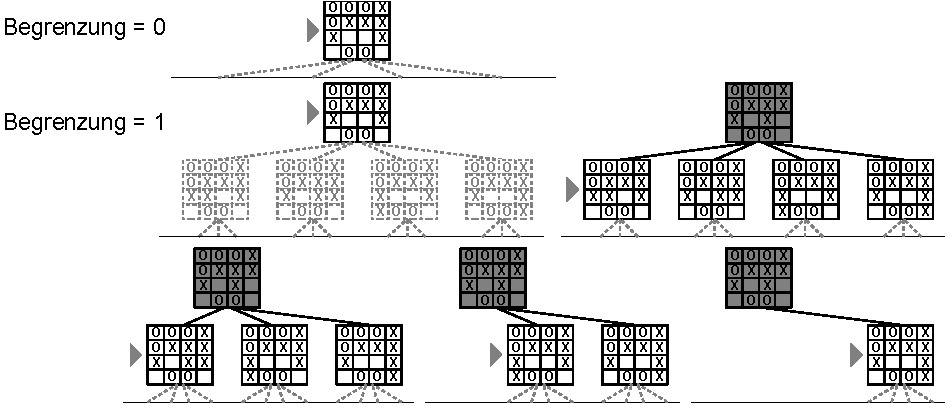
\includegraphics[scale = 0.9]{inhalt/abbildungen/iterative_deepening_tictactoe.pdf}
  \caption{TODO }
  \label{fig:minimax_tictactoe}
\end{figure}  
 
\paragraph{Die Breitensuche} expandiert (erweitert oder vergrößert) zu erst alle Nachfolger (Knoten eines Suchbaums) die in derselben Tiefe liegen, beginnend mit dem Wurzelknoten. Sind alle Nachfolger einer Tiefe expandiert, dann werden deren Nachfolger nacheinander expandiert. Diesen Schritt wiederholt die Breitensuche bis ein gesuchtes Ergebnis gefunden wird. \\

\paragraph{Die Tiefensuche} expandiert zuerst die tiefsten Knoten des Suchbaums(Depth-first). Erreicht die Tiefensuche einen Endknoten der nicht dem gesuchten Ergebnis entspricht, dann werden die alternativen Knoten des letzten expandierten Knotens, der sich eine Tiefenebene höher befindet, expandiert. \\

Kombinieren wir diese beiden uninformierten Suchverfahren miteinander und mit einer Grenze für die Suchtiefe, erhalten wir die iterative Tiefensuche. Diese expandiert zuerst die Nachfolger des Wurzelknotens der Suchtiefe 1. Sind alle Knoten auf dieser Ebene expandiert, dann wird die Schranke für die aktuelle Suchtiefe um 1 erhöht (Iteration) und die Knoten der Suchtiefe 2 werden expandiert. Diese Schritte wiederholt die Tiefensuche bis ein Ziel gefunden wird.  

\paragraph{Anwendung} findet die iterative Tiefensuche bei der Zugsortierung für die Verbesserung des Alpha-Beta Suchbaumkürzens. 


\subsection{Übergangstabelle}
Eine Übergangstabelle (eng. transition table) ist eine Tabelle in der Spielsituationen mit verschiedenen Attributen gespeichert werden (vgl. \cite[215\psq]{Russell}). Übergänge sind der Grund dafür, dass der gleiche Spielzustand durch unterschiedliche Spielzugsequenzen auftritt (siehe Abbildung \ref{fig:transitionen_tictactoe}). Folgende Attribute werden in der Übergangstabelle gespeichert: der Spielzustand, die Alpha-Beta Werte, der bestmögliche Halbzug, der Nutzen und welcher Spieler gerade setzen muss. Alle Attribute beziehen sich auf den gespeicherten Spielzustand z.B. der bestmögliche berechnete Halbzug der für den gespeicherten Spielzustand möglich ist. \\

\begin{figure}[!htbp]
  \centering
  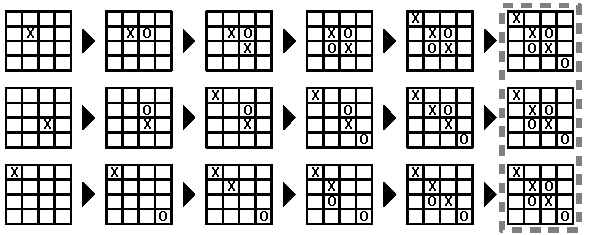
\includegraphics{inhalt/abbildungen/transitionen_tictactoe.pdf}
  \caption{Drei verschiedene Spielzugsequenzen die alle zum selben Spielzustand führen.}
  \label{fig:transitionen_tictactoe}
\end{figure} 

Übergänge innerhalb des Suchbaums verursachen Redundanzen. Für jede dieser Redundanzen wird eine erneute Suche durchgeführt, falls diese nicht durch Alpha-Beta-Kürzung abgeschnitten werden. Sollten diese Übergänge vermieden werden können, dann würde sich die Rechenzeit der Suchverfahren weiter verringern, weil weniger Spielzustände durchsucht bzw. expandiert werden müssen. Wie können wir Spielzustände in einer Übergangstabelle abspeichern? \\

\myparagraph{Zobrist Hash}
Wenn ein Computerprogramm einen Gegenstand in einer großen Tabelle speichert, muss die Tabelle zwangsläufig durchsucht werden, um den Gegenstand wiederzuverwenden bzw. zu referenzieren. Dies gilt solange, bis eine Tabellendresse aus dem Gegenstand selbst, in systematischer weise, berechnet werden kann. Eine Funktion die Gegenstände in Adressen umwandelt ist ein Hash-Algorithmus, und die daraus resultierende Tabelle ist eine Hashtabelle \cite[3]{Zobrist}. \\

\begin{figure}[!htbp]
  \centering
  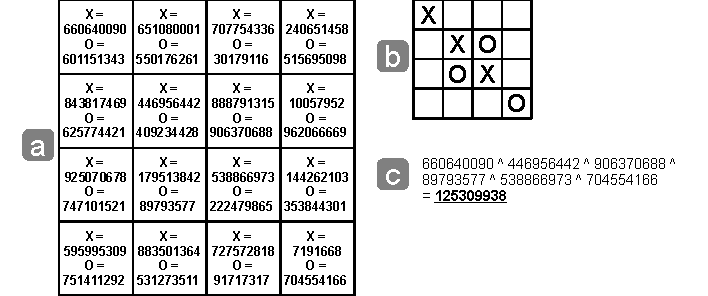
\includegraphics[scale = 1.3]{inhalt/abbildungen/zobrist_hash_tictactoe.pdf}
  \caption{Zobrist Hashing von Spielzuständen.}
  \label{fig:zobrist_hash_tictactoe}
\end{figure} 


In Abbildung \ref{fig:zobrist_hash_tictactoe} wird das Zobrist Hash Verfahrens auf den redundanten Spielzustand aus Abbildung \ref{fig:transitionen_tictactoe} angewendet. (\ref{fig:zobrist_hash_tictactoe} a) Wir weisen jedem Spielfeld zwei zufällige ganzzahlige Werte zu im Bereich von 0 bis maximal $1 \times 10^{9}$. Einen zufälligen Wert für den Kreuzspielstein an dieser Position und einen für den Kreisspielstein. Das 4x4 Tic Tac Toe Spielbrett sollte insgesamt 32 verschiedene Werte erhalten. (\ref{fig:zobrist_hash_tictactoe} b) Dieser Spielzustand soll in einen Zobrist-Hash umgewandelt werden. \\

(\ref{fig:zobrist_hash_tictactoe} c) Der Zobrist-Hash berechnet sich wie folgt, ist die aktuelle Position mit einem Kreuzspielstein oder einem Kreisspielstein besetzt, dann wähle den entsprechenden Wert aus (\ref{fig:zobrist_hash_tictactoe} a). Dies wiederhole für jedes besetzte Spielfeld. Auf den bereits ermittelten Wert und den hinzukommenden Wert wird ein exklusives bitweises Oder (XOR) angewendet. In Python ist das Zeichen für die Funktion des exklusiven bitweisen Oder ein Zirkumflex (siehe Operatoren in der Berechnung \ref{fig:zobrist_hash_tictactoe} c). Das Ergebnis ist eine Adresse die exakt den Spielzustand (\ref{fig:zobrist_hash_tictactoe} b) referenziert. \\

Spielzustände die gerade expandiert werden, können in die Übergangstabelle eingetragen werden, sollten diese nicht bereits in der Tabelle vorhanden sein. Ist dieser Spielzustand bereits in der Tabelle vorhanden, dann können die vorgeschlagenen besten Halbzüge aus der Tabelle ausgelesen und angewendet werden. \\

\subsection{Heuristik}
\label{subsec:Heuristik}
Eine Heuristik oder Bewertungsfunktion berechnet einen Nutzwert für einen gegebenen Spielzustand. Dieser Nutzwert gibt an, wie "wertvoll" diese Spielsituation hinsichtlich eines Sieges ist, sprich sie gibt an ob der Spieler in diesem Spielzustand eher gewinnen oder verlieren könnte. Trotz aller Optimierungen des Minimax Verfahrens (Alpha-Beta, Zugsortierung, Vermeidung von Redundanzen) wäre die Rechenzeit, für den zu durchsuchenden Baum, immer noch enorm hoch. Reale Zeitbeschränkungen z.B. bei Schach Spielen erlauben ein überaus langes Berechnen ohnehin nicht. Die Lösung ist das verwenden einer Heuristik. Der Kompromiss bei einer Heuristik ist: das Ergebnis wird geschätzt und ist nicht mehr sicher, aber die Suche kann nach einem Zeitkriterium abgebrochen werden und die beste bisher gefundene Lösung wird zurückgegeben. Sollte die Bewertungsfunktion für einen Spielzustand z.B. einen sehr hohen Wert berechnen, dann besagt dieser, der Spieler der diesen Spielzustand erreicht wird wahrscheinlich gewinnen. \\

Die Qualität einer Heuristik ist ausschlaggebend für die Spielerischen Fähigkeiten eines Programms. Ein Programm welches, durch eine schlechte Stellungsbewertung (Heuristik) einen fatalen Spielzug des Gegners übersieht oder ignoriert, würde gegen ein Programm verlieren, welches diese Stellungen (Spielzustände) erkennt und ausnutzt bzw. entsprechend verhindert. Eine Bewertungsfunktion B(s) für ein Schachspiel enthält folgende Elemente, wobei s der Parameter für den Spielzustand ist\cite[119]{Ertel}: \\

B(s) = $a_1$ x Material +  $a_2$ x Bauernstruktur + $a_3$ x Königssicherheit \\
\tab \tab + $a_4$ x Springer im Zentrum + $a_5$ x Läufer Diagonalabdeckung + ..., \\ 

das mit Abstand wichtigste Feature (Merkmal) "Material" nach der Formel \\

\tab \tab Material = Material(eigenes Team) - Material(Gegner) \\

Material(Team) = Anzahl Bauern(Team) x 100 + Anzahl Springer(Team) x 300 \\
\tab \tab \tab + Anzahl Läufer(Team) x 300 + Anzahl Türme(Team) x 500 \\
\tab \tab \tab + Anzahl Damen(Team) x 900 \\

Diese Schach Heuristik ist entstanden aus der Zusammenarbeit von Schachexperten und Wissensingenieuren. Die Schachexperten verfügen über Wissen und Erfahrungen bezüglich des Schachspiels, der Strategien, guter Zugstellungen und schlechter Zugstellungen. Der Wissensingenieur hat die meist sehr schwierige Aufgabe dieses Wissen in eine, für ein Programm, anwendbare Form zu bringen (vgl. \cite[118]{Ertel}). \\

Eine Heuristik ist stark Abhängig von ihrer Grundlage, d.h. eine Heuristik die für ein Schachspiel konzipiert wurde, berücksichtigt die Spielfiguren, das Spielfeld und die Spielregeln des Schachspiels. Wir können diese Heuristik nicht direkt auf Reversi oder Tic Tac Toe anwenden, weil eine Schach Heuristik nicht auf andere Spiele angewendet werden kann. Eine Reversi Heuristik kann z.B. auch nicht für das Spielen eines Tic Tac Toe Spiels verwendet werden. Es ist uns jedoch möglich das Konzept, sprich die Essenz der Heuristik Entwicklung, aus dieser Beispielheuristik für Schachspiele zu entnehmen und auf die Heuristik Entwicklung für Reversi und Tic Tac Toe anzuwenden. \\

Mehr zum Thema Heuristik Entwicklung in Kapitel \ref{cha:Modellierung und Entwurf} Modellierung und Entwurf, in diesem Kapitel werden wir ähnlich der gerade vorgestellten Heuristik, eigene Bewertungsfunktionen für Tic Tac Toe und Reversi entwerfen und in Kapitel \ref{cha:Implementierung} Implementierung, werden die modellierten Bewertungsfunktionen praktisch angewendet. \\

\section{Verstärkendes Lernen(Reinforcement Learing)}
\label{sec:Verstärkendes Lernen}
Verstärkendes oder auch bestärkendes Lernen beschäftigt sich mit dem Problem, dass ein Entscheidung treffender Agent, innerhalb einer ihm unbekannten Umgebung, Aktionen (Entscheidungen) ausführen muss (Abbildung \ref{fig:agent_umgebung}). Das Ziel des Agenten ist es, einen nummerischen Wert zu maximieren. Dieser Wert wird durch numerische Belohnung oder Bestrafung verändert. Der Agent lernt das Verhältnis zwischen den möglichen Aktionen in einem Zustand und deren numerischer Bewertung. Führt eine Aktion in einem Zustand mehrfach zu wiederholt herausragender positiver Bewertung, dann wird der Agent diese Aktion in diesem Zustand erneut ausführen. \\

\begin{figure}[!htbp]
  \centering
  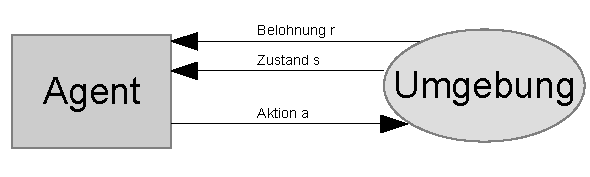
\includegraphics[scale = 1.4]{inhalt/abbildungen/agent_umgebung.pdf}
  \caption{Der Agent und seine Wechselwirkung mit der Umgebung. Die Darstellung des Agenten und der Umgebung wird in verschiedenen Fachbüchern, die das  verstärkenden Lernen behandeln, sehr ähnlich realisiert \cite[398]{Alpaydin} und \cite[290]{Ertel}.}
  \label{fig:agent_umgebung}
\end{figure} 

Wie kann sich der Agent die Bewertungen seiner Aktionen merken und sich daran erinnern? Dies ist möglich, weil der Agent über einen Erfahrungsspeicher verfügt z.B. eine Übergangstabelle. Der Agent schreibt neue Zustände, ausgeführte Aktionen und mögliche Bewertungen der Aktionen in die Tabelle. Vorher prüft der Agent ob der Zustand bereits in der Tabelle eingetragen ist. Existiert dieser Zustand in der Tabelle, hat der Agent Erfahrung in diesem Zustand gesammelt und kann diese nutzen und anpassen. \\
 
Bei realen Problemen, wie dem lernen von Schach oder Reversi, erfolgt eine Belohnung oder Bestrafung nicht direkt nach einer Aktion des Agenten (verspätete Belohnung, eng. delayed reward). Erst nach Abschluss einer Partie, also nach einer Sequenz von bestimmten Aktionen, endet das Spiel und der Agent wird für einen Sieg belohnt oder für eine Niederlage bestraft. Eine große Schwierigkeit ist diese verspätete Belohnung am Ende einer Aktionssequenz auf die einzelnen Aktionen des Agenten aufzuteilen. Dieses Problem ist bekannt als Anerkennungszuweisung Problem (eng. credit assignment problem). \\

\subsection{Ein Agent im Labyrinth}
Nehmen wir an es existiere folgender Agent. Dieser Agent kann vier Aktionen ausführen, bewege dich nach oben, unten, rechts oder links. Er wird in einem ihm unbekannten Labyrinth ausgesetzt. Das Labyrinth ist die Umgebung und die Zustände der Umgebung verändern sich durch die Aktionen des Agenten, das heißt verändert der Agent seine Position innerhalb des Labyrinths, dann wechselt er von einem Ausgangszustand, durch eine Aktion, in einen neuen Zustand der Umgebung. \\

Der Agent lernt also, dass die Aktion 'bewege dich nach oben' den Ausgangszustand in einen neuen Zustand transformiert. Führt der Agent die Aktion 'bewege dich nach oben' aus, dann ist jedoch die Zustandsveränderung abhängig von der individuellen Umgebung in der sich der Agent befindet. In einem Labyrinth kann der Agent nicht immer alle seiner vier Aktionen ausführen, denn er ist umringt von Mauer die seinen Aktionsradius beschränken. Würde er trotzdem eine unzulässige Aktion ausführen, dann verändert sich der Zustand der Umgebung nicht, denn der Agent würde sprichwörtlich "gegen die Wand laufen". \\

Nach einer endlichen Sequenz von Aktionen gelingt es dem Agenten den Ausgang des Labyrinths zu erreichen und er erhält eine nummerische Belohnung entsprechend der Anzahl seiner ausgeführten Aktionen. Die nummerische Belohnung wird höher, je weniger Aktionen der Agent benötigt hat, um den Ausgang des Labyrinths zu erreichen. Die Aktionen die der Agent bei erreichen des Ausgangs ausgeführt hat, werden im ersten Versuch und vielleicht in den Nachfolgenden Versuchen wahrscheinlich nicht optimal sein. Nicht optimal in dem Sinne, dass die Aktionssequenz nicht die kürzeste sein wird. Der Agent kann den Wert für die nummerische Belohnung maximieren, indem er eine optimale Strategie entwickelt, die den kürzesten Pfad findet. Eine optimale Strategie die für jeden möglichen Zustand eindeutig definiert, welche Aktion er durchführen muss, um so wenig wie möglich Aktionen zu verwenden und den Ausgang zu erreichen. \\

\subsection{Mathematische Formulierung der optimalen Strategie}
Der Zustand $s_t \in S$ beschreibt die Position eines Agenten in einer Umgebung zu einem festgelegten Zeitpunkt t. S ist eine menge von möglichen Zuständen. Die Aktion $a_t \in A$ wird vom Agenten, zum Zeitpunkt t, ausgeführt und verändert die Umgebung(siehe Abbildung \ref{fig:agent_umgebung}). Diese Aktion überführt den vorherigen Zustand $s_t$ in einen neuen zustand $s_t+1$. Der neue Zustand $s_t+1 = \delta(s_t, a_t)$ wird von der Übergangsfunktion $\delta$ bestimmt. Die Übergangsfunktion wird von der Umgebung bestimmt und kann von dem Agenten nicht beeinflusst werden. Führt ein Agent eine Aktion a in einem Zustand s zu einem Zeitpunkt t aus, dann erhält der Agent eine direkte Belohnung(engl. immediate reward) $t_t = r(s_t, a_t)$. Diese direkte Belohnung ist abhängig von dem aktuellen Zustand und der ausgeführten Aktion\cite[290]{Ertel}. \\

\subsection{Überwachtes \acs{vs.} verstärkendes Lernen}
Im Gegensatz zu den Lernverfahren beim überwachten Lernen fehlt dem Agenten beim verstärkenden Lernen ein Lehrer der dem Agenten genau sagt ob seine Aktion richtig oder falsch ist. Zudem wäre ein Lehrer, der dem Agenten für jeden Zustand genau sagt welches die richtige Aktion ist, sehr kostspielig. Oftmals ist für einen Zustand gar keine optimale Aktion möglich, erst die Aneinanderreihung von Aktionen und Zustandsübergängen kann optimal sein oder optimiert werden\cite[\acs{vgl.} 397]{Alpaydin}. \\

Ein überwachtes Lernverfahren wird zuerst mittels eines Trainingssets kontrolliert belehrt. Das Trainingsset für ein überwachtes Lernverfahren besteht aus verschiedenen Eigenschaften (Features) und einer den Eigenschaften zugeordneten Klasse beziehungsweise Zielvariable (Target Variable). Die Qualität der Zielwerte kann mittels Testsets ermittelt werden. Ein Testset ist ein Datenset bestehend aus Eigenschaften ohne die dazugehörigen Klassen. Abbildung \ref{fig:vogel_spezies} zeigt, wie ein Trainingsset aussehen könnte\cite[8]{Harrington}. Die Spalten Gewicht, Flügelspanne, Schwimmhäute und Rückenfarbe sind die Eigenschaften und die Spalte Spezies beinhaltet die Zielvariablen. Das überwachte Lernverfahren lernt mittels des Trainingsdatensets die Beziehungen zwischen den Eigenschaften und der Klassen. \\

\begin{figure}[!htbp]
  \centering
  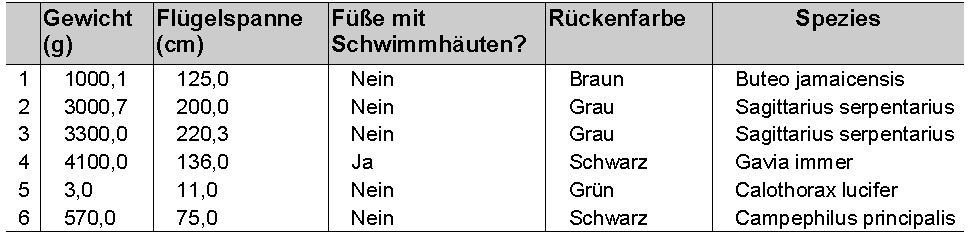
\includegraphics[scale = 0.89]{inhalt/abbildungen/vogel_spezies.pdf}
  \caption{Vogelspezies Klassifikation basierend auf vier Eigenschaften}
  \label{fig:vogel_spezies}
\end{figure} 

Verstärktes Lernen umfasst die Probleme, bei denen in der Regel kein solches Trainingsdatenset vorliegt, welches genau festlegt ob eine Aktion in einem Zustand korrekt oder falsch ist. Bezogen auf ein Testdatenset wäre eine Aktion des Agenten, dass nennen einer Klasse hinsichtlich der gelernten Zusammenhänge aus den Trainingsdaten. Teilt man die Anzahl der korrekten Vorschläge durch die Anzahl aller Versuche, dann erhält man eine Kennzahl für die Qualität der Vorhersage. Sind alle Klassen der Testinstanzen richtig vorhergesagt, dann ist die Kennzahl genau Eins. Jede Zeile eines Testsets und jede Zeile eines Trainingssets ohne die Zielvariablen ist eine Instanz. Verstärkendes Lernen kann trotzdem vom überwachten Lernen profitieren, denn es ist möglich den Agenten in der Anfangsphase des verstärkten Lernens explizit zu programmieren und ihn dadurch auf bestimmte Auffälligkeiten oder Muster aufmerksam zu machen. Ist es zu kompliziert dies explizit zu programmieren, dann kann auch ein Mensch dem Agenten die richtigen Aktionen vorgeben. \\

Sehr nützlich werden diese beiden Unterstützungen der Anfangsphase des verstärkenden Lernens, sobald die Dimensionen der Umwelt oder des Agenten eine bestimmte Größe überschreiten. Eine Aktionsdimension kann sehr wenige Aktionen beinhalten zum Beispiel die vier Aktionen bewege dich nach oben, unten, rechts oder links. Roboter die dem Menschen nachempfunden sind verfügen über bis zu 50 verschiedene Motoren für die einzelnen Gelenke. Diese müssen gleichzeitig angesteuert werden, was zu einem 50-dimensionalen Zustandsraum und einem 50-dimensionalen Aktionenraum führt\cite[\acs{vgl.} 305\psq]{Ertel}. Bei solch großen Dimensionen können die Laufzeiten einiger verstärkender Lernverfahren massiv ansteigen, bis sie praktisch nicht mehr anwendbar sind. Gerade in der Anfangsphase des verstärkten Lernens kann darum ein Eingriff mittels überwachtem Lernen sehr Laufzeit schonend sein.